\section{Instalar ROS 2}
Ahora vamos a instalar ROS 2 en la raspberry pi (específicamente instalamos ROS 2 en la micro SD de la raspberry pi, pues esa es su memoria secundaria, como su disco duro). %Debemos de insertar la micro SD en la raspbery pi y conectarnos remotamente (via ssh) a la raspberry.  

\subsection{Conocer la IP de la Raspberry}
Vamos a enfuchar la raspberry a la luz para encenderla. Luego conectaremos un teclado, un mouse y una pantalla en los puertos correspondientes de la raspberry. El teclado y mouse se conectarán a puertos USB, y la pantalla al puerto HDMI. 

\begin{figure}[H]
    \centering
    \makebox[\textwidth][c]{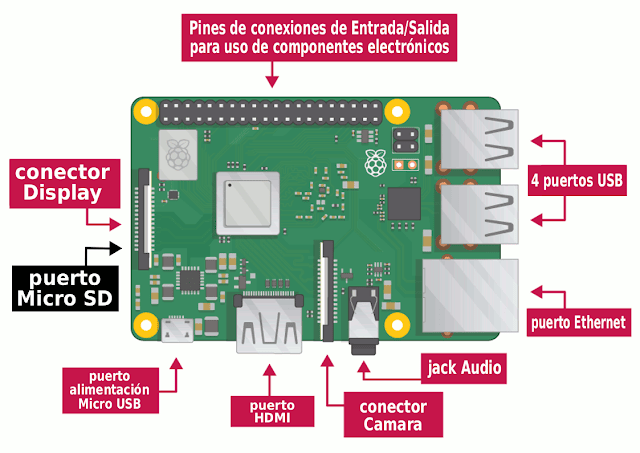
\includegraphics[width=0.9\textwidth]{imagenes/puertos-raspberry.png}}
    \caption{Puertos y partes de una raspberry.}
    \label{fig:mi_imagen}
\end{figure}

Una vez hecho eso, se debería mostrar en la pantalla el escritorio de la raspberry. Con el acceso al escritorio de la raspberry, nos conectamos al wifi. Luego, consultamos nuestra dirección IP con el comando \texttt{ifconfig}. 

Y así podemos conocer la dirección IP de la raspberry pi. Esto es útil pues nos permitirá conectarnos remotamente a la placa sin tener que conectar una pantalla, un teclado y un mouse cada vez.

\subsection{Ahora sí, procedemos a instalar ROS 2 en la Raspberry}
Para proceder con la instalación de ROS 2 en la rapsberry, vamos a conectarnos remotamente a esta. Lo haremos con el protocolo ssh. En nuestra computadora, ejecutamos el siguiente comando en terminal:

\begin{center}
    \begin{Verbatim}[gobble=4]
    ssh <nombre del usuario>@<dirección IP>
    \end{Verbatim}
\end{center}

Dondo $<$nombre de usuario$>$ es el nombre del usuario al cual queremos conectarnos, y $<$dirección IP$>$ es la dirección IP del host al cuál queremos conectarnos.

Una vez dentro de la raspberry, vamos a crear un nuevo usuario llamado \textit{paquito}. Esto es importante, pues el compilado de ROS 2 que vamos a instalar en la raspberry funciona obligatoriamente con un usuario \textit{paquito}. Entonces, creamos el usuario con el siguiente comando:

\begin{center}
    \begin{Verbatim}[gobble=4]
    sudo adduser paquito    
    \end{Verbatim}
\end{center}

Y procedemos a cambiarnos al usuario \textit{paquito} con:

\begin{center}
    \begin{Verbatim}[gobble=4]
    sudo su paquito    
    \end{Verbatim}
\end{center}

Ahora sí, dentro del usuario \textit{paquito}, lo que primero vamos a hacer es seguir los pasos de la página de Quetzalcoatl en el apartado de Raspberry Pi OS, al cual se puede acceder \href{https://quetzalcoatl.fciencias.unam.mx/taller-de-robotica/index.php/recursos-para-organizadores/raspberrypi-os-para-el-taller/}{acá}. Esos pasos son para agregar ciertas dependecias y hacer ciertas configuraciones antes de instalar ROS 2 en la raspberry.

Una vez que terminemos esos pasos, debemos de descargar un archivo comprimido \texttt{.tar.gz} dando click en la palabra Jazzy (que se muestra en la siguiente figura) de la página.

\begin{figure}[H]
    \centering
    \makebox[\textwidth][c]{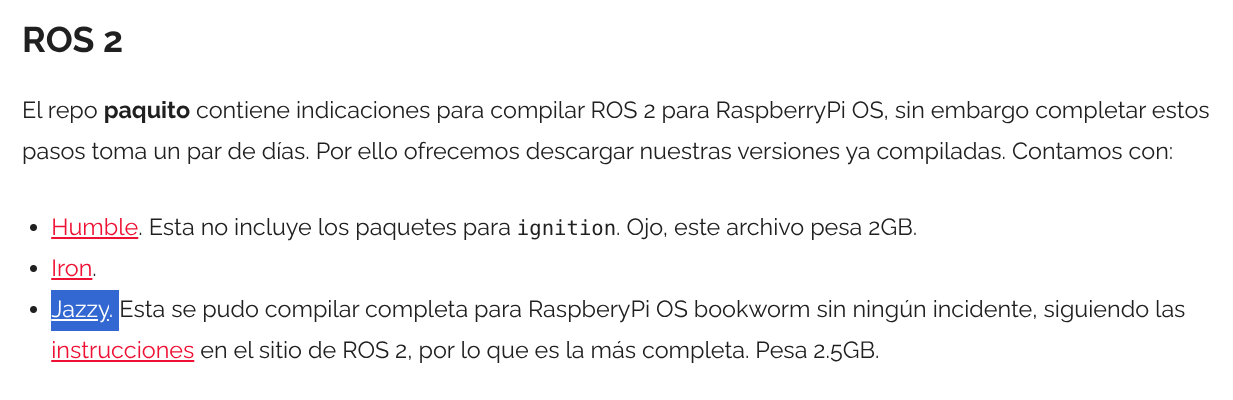
\includegraphics[width=1.2\textwidth]{imagenes/targzjazzy.png}}
    \caption{Dar Click en Jazzy para obtener el ROS 2 compilado para Raspberry}
    \label{fig:mi_imagen}
\end{figure}

En la raspberry pi, en la ruta del usuario, se debe descomprimir el archivo descargado anteriormente con el comando \texttt{tar -xzvf archivo.tar.gz}.

\begin{center}
    \begin{Verbatim}[gobble=4]
        paquito@raspberrypi:~ $ tar -xzvf archivo.tar.gz
    \end{Verbatim}
\end{center}

Ahora, vas a tener una nueva carpeta llamada \texttt{ros2\_jazzy} dentro de la carpeta del usuario paquito. Esa carpeta ya es ROS, con esa carpeta ya tienes instalado ROS en la raspberry. Cuando instalamos ROS en una computadora normal (no raspberry) con ubuntu, la instalación de ROS se hizo en la carpeta \texttt{jazzy} en la ruta \texttt{/opt/ros/}, es decir, en nuestras computadoras tenemos a ROS instalado en \texttt{/opt/ros/jazzy/}. Sin embargo, la raspberry tiene instalado ROS en \texttt{/home/paquito/ros2\_jazzy}. Por tanto, para activar el underlay en la raspberry, debemos de escribir el siguiente comando:

\begin{center}
    \begin{Verbatim}[gobble=4]
    source ~/ros2_jazzy/install/local_setup.bash    
    \end{Verbatim}
\end{center}

Para no tener que activar el underlay todo el tiempo en la raspberry pi, vamos a guardar el comando de activación de underlay en el archivo \texttt{.bashrc}, para hacerlo, ejecutaremos el siguiente comando:%\\\verb|echo "source ~/ros2_jazzy/install/local_setup.bash" >> ~/.bashrc|

\begin{center}
    \begin{Verbatim}[gobble=4]
    echo "source ~/ros2_jazzy/install/local_setup.bash" >> ~/.bashrc    
    \end{Verbatim}
\end{center}

\begin{center}
    \begin{Verbatim}[gobble=4]
    paquito@raspberrypi:~ $ echo "source ~/ros2_jazzy/install/local_setup.bash" \
    >> ~/.bashrc
    \end{Verbatim}
\end{center}

Para activar overlays, va a ser exactamente igual que en nuestras pc's. En la carpeta del espacio de trabajo, ejecutar \texttt{source install/local\_setup.bash}.